Lo standard ISO/IEC 9126 stabilisce una serie di linee guida mirate al miglioramento delle qualità del software sviluppato.

\begin{figure}[H]
  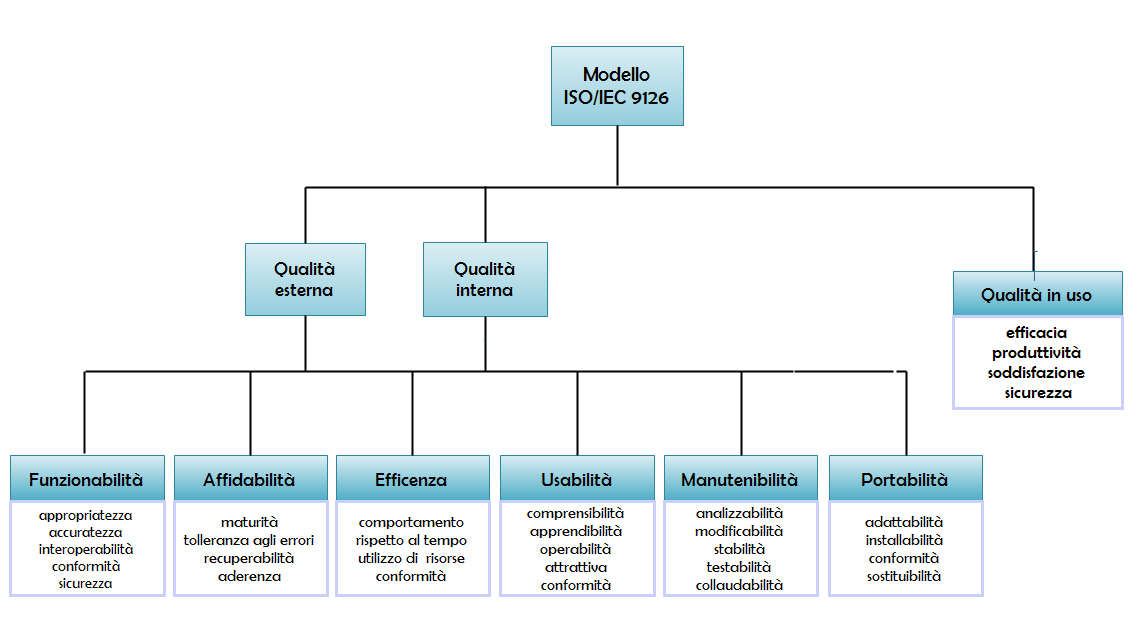
\includegraphics[width=\linewidth]{sez/App_Qualita/grafico_9126.png}
  \caption{Rappresentazione grafica di ISO/IEC 9126 [Wikipedia]}
  \label{fig:9126}
\end{figure}

Come presentato in \autoref{fig:9126}, ISO/IEC 9126 prescrive indicazioni su:
\begin{itemize}
	\item \textbf{Qualità interna: }è misurata sul software non eseguibile, come, ad esempio il codice sorgente. Le misure effettuate (appendice \cref{app:misure}) permettono di avere una buona previsione della qualità esterna. Le metriche usate dal gruppo \gruppo \space sono reperibili in \cref{sec:metriche}.
	\item \textbf{Qualità esterna: }è misurata tramite l'analisi dinamica su software eseguibile. Le misure effettuate (appendice \cref{app:misure}) permettono di avere una buona previsione della qualità in uso prodotto. Le metriche usate dal gruppo \gruppo \space sono le tecniche di analisi dinamica reperibili in \cref{sec:metriche}.
	\item \textbf{Qualità in uso: }definita in base all'esperienza utente. Sono da perseguire i seguenti obiettivi:
		\begin{itemize}
			\item Efficacia;
			\item Produttività;
			\item Soddisfazione;
			\item Sicurezza.
		\end{itemize}
\end{itemize}

ISO/IEC 9126 definisce inoltre una serie di requisiti da soddisfare per produrre software di qualità:
\begin{itemize}
	\item \textbf{Funzionalità: }capacità di un prodotto software di soddisfare le esigenze stabilite (vedi \AdR);
	\item \textbf{Affidabilità: }capacità di un prodotto di mantenere un determinato livello di prestazioni in date condizioni d'uso per un certo periodo;
	\item \textbf{Efficienza: }capacità di un prodotto software di eseguire il proprio compito minimizzando il numero di risorse usate;
	\item \textbf{Usabilità: }capacità del prodotto software di essere utilizzato, capito e studiato dall'utente a cui è rivolto;
	\item \textbf{Manutenibilità: }capacità del prodotto software di evolvere mediante modifiche, correzioni e miglioramenti;
	\item \textbf{Portabilità: }capacità del prodotto software di funzionare ed essere installato su più ambienti hardware e software.
\end{itemize}